% Figure 1: attention kernel latency, Inkling-turbo against every day-0 path.
%
% Build: tectonic docs/figures/fig1_latency.tex
%
% Every value is measured on one H100 SXM5 (sm_90), session 25,
% torch 2.11 / cu130. Sources:
%   journal/remote/microbench_attn_day0_session25_h100.json      (ours)
%   journal/remote/microbench_attn_scoremod_session25_h100.json  (day-0)
% A missing point means that pairing was never run. Nothing is filled in.
%
% A dot plot, not bars: on a log axis bar length is not proportional to
% value, so bars would misrepresent the ratios.

\documentclass[border=14pt]{standalone}
% Shared style for all Inkling-turbo figures.
% Included by each standalone figure so they read as one family.
\usepackage{tikz}
\usepackage{pgfplots}
\pgfplotsset{compat=1.18}
\usetikzlibrary{calc,plotmarks,backgrounds}

% palette
\definecolor{ours}{HTML}{0B6E6A}     % our kernel
\definecolor{floorc}{HTML}{64748B}   % the biasless floor
\definecolor{prod}{HTML}{C2410C}     % the path vLLM ships
\definecolor{altA}{HTML}{9A3412}     % other day-0 paths
\definecolor{altB}{HTML}{78350F}
\definecolor{ink}{HTML}{111827}      % text
\definecolor{guide}{HTML}{DDE1E6}    % grid
\definecolor{band}{HTML}{F4F6F8}     % group banding
\definecolor{okc}{HTML}{15803D}      % validated
\definecolor{partc}{HTML}{B45309}    % partial

% shared axis look: no frame, no ticks, faint grid, small labels
\pgfplotsset{
  inkling/.style={
    scale only axis,
    axis line style={draw=none},
    tick style={draw=none},
    grid style={line width=0.45pt, color=guide},
    xticklabel style={font=\scriptsize, color=ink!62},
    yticklabel style={font=\scriptsize, color=ink!88},
    xlabel style={font=\footnotesize, color=ink!85},
    ylabel style={font=\footnotesize, color=ink!85},
    clip=false,
  },
}

% figure title + standfirst, placed above a named axis
\newcommand{\figtitle}[3]{%
  % #1 axis name, #2 title, #3 standfirst
  \node[anchor=north west, font=\bfseries, color=ink]
    at ($(#1.north west)+(\titleoffset,\titletop)$) {\large #2};
  \node[anchor=north west, font=\scriptsize, color=ink!58,
        text width=\standfirstwidth]
    at ($(#1.north west)+(\titleoffset,\titlesub)$) {#3};
}


\def\titleoffset{-3.55cm}
\def\titletop{1.75cm}
\def\titlesub{1.30cm}
\def\standfirstwidth{16.6cm}

\begin{document}
\sffamily
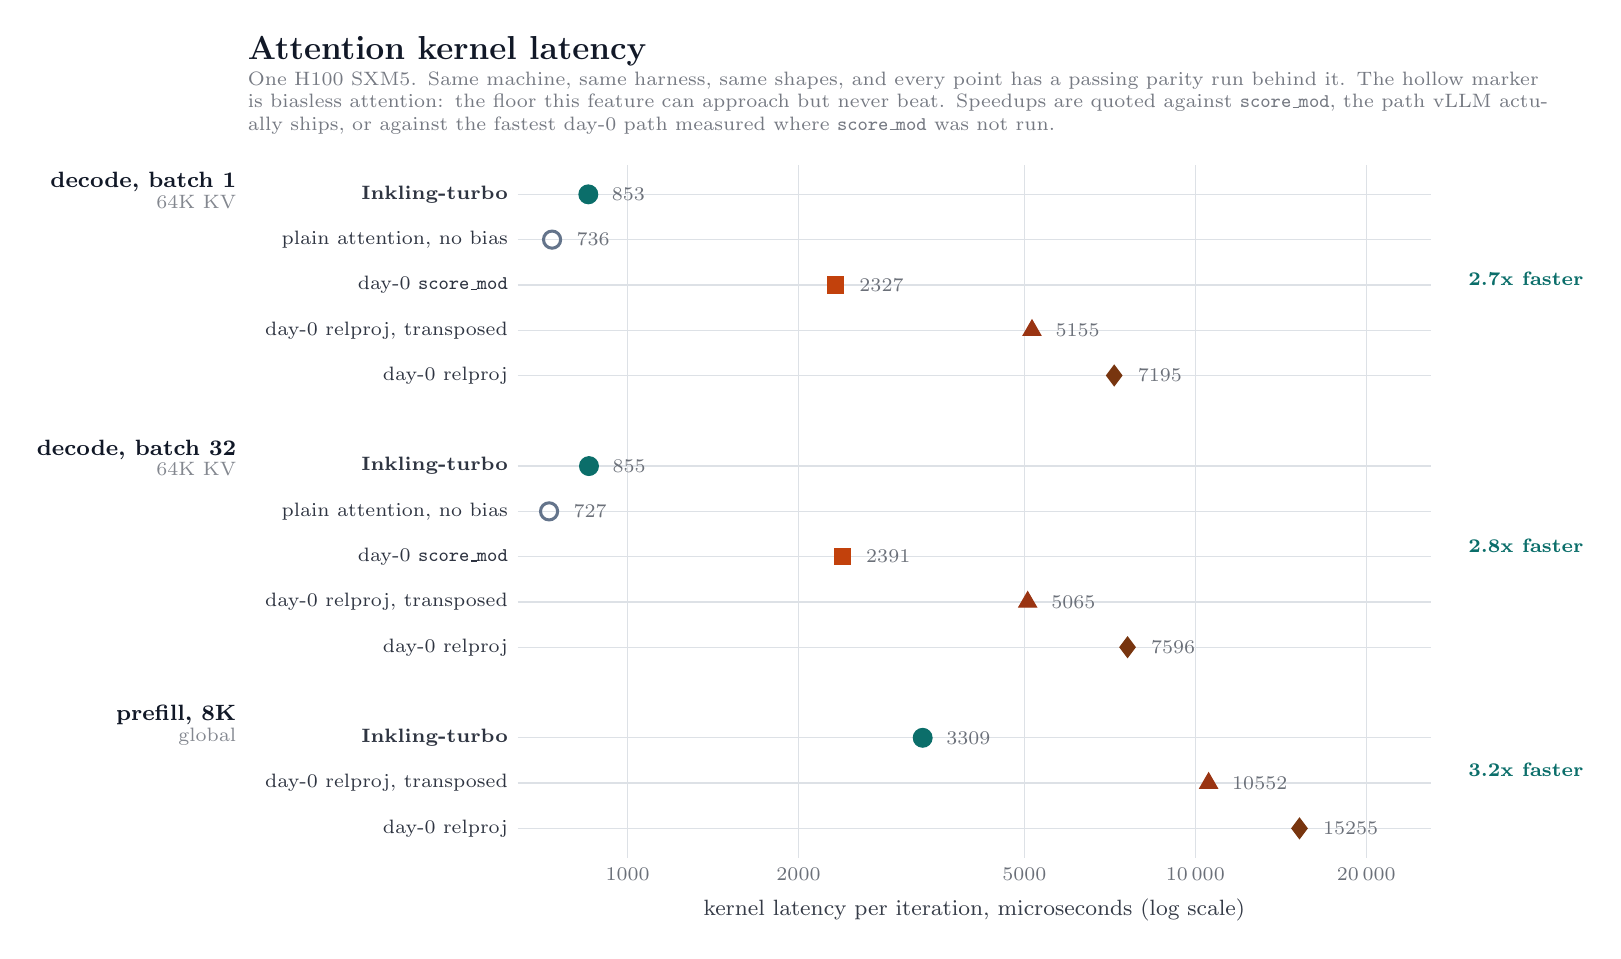
\begin{tikzpicture}[font=\sffamily]

\begin{axis}[
  inkling,
  name=A,
  width=11.6cm, height=8.8cm,
  xmode=log, log basis x=10,
  xmin=640, xmax=26000,
  xtick={1000,2000,5000,10000,20000},
  xticklabels={1000,2000,5000,{10\,000},{20\,000}},
  xlabel={kernel latency per iteration, microseconds (log scale)},
  ymin=0.35, ymax=15.65,
  ytick={1,2,3,5,6,7,8,9,11,12,13,14,15},
  yticklabels={
    {day-0 relproj},
    {day-0 relproj, transposed},
    {\textbf{Inkling-turbo}},
    {day-0 relproj},
    {day-0 relproj, transposed},
    {day-0 \texttt{score\_mod}},
    {plain attention, no bias},
    {\textbf{Inkling-turbo}},
    {day-0 relproj},
    {day-0 relproj, transposed},
    {day-0 \texttt{score\_mod}},
    {plain attention, no bias},
    {\textbf{Inkling-turbo}}},
  ymajorgrids, xmajorgrids,
  point meta=explicit symbolic,
  nodes near coords,
  nodes near coords style={font=\scriptsize, color=ink!62, anchor=west,
                           xshift=5pt},
]

\addplot[only marks, mark=*, mark size=3.4pt, color=ours]
  coordinates {(852.6,15) [853] (854.8,9) [855] (3308.8,3) [3309]};

\addplot[only marks, mark=o, mark size=3.1pt, line width=1.1pt, color=floorc]
  coordinates {(736.0,14) [736] (727.2,8) [727]};

\addplot[only marks, mark=square*, mark size=2.9pt, color=prod]
  coordinates {(2326.6,13) [2327] (2391.2,7) [2391]};

\addplot[only marks, mark=triangle*, mark size=3.7pt, color=altA]
  coordinates {(5154.7,12) [5155] (5065.1,6) [5065] (10551.5,2) [10552]};

\addplot[only marks, mark=diamond*, mark size=3.7pt, color=altB]
  coordinates {(7194.5,11) [7195] (7595.5,5) [7596] (15254.6,1) [15255]};

\end{axis}

% ---- workload group labels
\node[anchor=east, font=\footnotesize\bfseries, color=ink, align=right]
  at ($(A.north west)+(-3.45cm,-0.32cm)$)
  {decode, batch 1\\[-2pt]{\scriptsize\mdseries\color{ink!52}64K KV}};
\node[anchor=east, font=\footnotesize\bfseries, color=ink, align=right]
  at ($(A.north west)+(-3.45cm,-3.72cm)$)
  {decode, batch 32\\[-2pt]{\scriptsize\mdseries\color{ink!52}64K KV}};
\node[anchor=east, font=\footnotesize\bfseries, color=ink, align=right]
  at ($(A.north west)+(-3.45cm,-7.12cm)$)
  {prefill, 8K\\[-2pt]{\scriptsize\mdseries\color{ink!52}global}};

% ---- speedup against the path vLLM ships
\node[anchor=west, font=\scriptsize\bfseries, color=ours]
  at ($(A.north east)+(0.35cm,-1.44cm)$) {2.7x faster};
\node[anchor=west, font=\scriptsize\bfseries, color=ours]
  at ($(A.north east)+(0.35cm,-4.84cm)$) {2.8x faster};
\node[anchor=west, font=\scriptsize\bfseries, color=ours]
  at ($(A.north east)+(0.35cm,-7.68cm)$) {3.2x faster};

\figtitle{A}{Attention kernel latency}{%
  One H100 SXM5. Same machine, same harness, same shapes, and every point has
  a passing parity run behind it. The hollow marker is biasless attention: the
  floor this feature can approach but never beat. Speedups are quoted against
  \texttt{score\_mod}, the path vLLM actually ships, or against the fastest
  day-0 path measured where \texttt{score\_mod} was not run.}

\end{tikzpicture}
\end{document}
